\newpage
\texHeader
\hypertarget{simpleDemo tex}{} 
\subsection{A first look at MOSL}

\begin{itemize}

\item[$\blacktriangleright$] You should immediately have 3 folders available in your project explorer -- Your metamodel project,
\texttt{DoubleLinkedListLanguage}, and \\ \texttt{DemoTestSuite} (Fig.~\ref{eclipse:texErrors}). Initially, you'll see a red exclamation mark indicating there
are errors, but once you give Eclipse a few seconds to refresh, all problems should be solved.

\vspace{1cm}

\begin{figure}[htp]
\begin{center}
  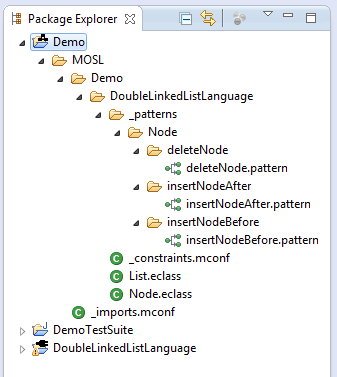
\includegraphics[width=0.5\textwidth]{eclipse_loadedTexDemo}
  \caption{Metamodel file structure}
  \label{eclipse:texErrors}
\end{center}
\end{figure}

\vspace{1cm}

\item[$\blacktriangleright$] That's it! You're all set up! But, while you're here, feel free to explore the ``Demo'' folder. It has the basic code that implements
this demo, and we recommend you take a brief look to get a feel for the the general syntax.

In the meantime, please do not rename, move, or delete anything.

\end{itemize}
